%% This is based on the leaflet.tex file present in the texlive-leaflet module
%% 
%% Copyright 2014 Ankur Sinha for the Fedora Marketing Team - marketing@lists.fedoraproject.org
% Please e-mail the marketing team if you have any questions with this document

\def\filename{fedora-flyer-server.tex}
\documentclass[
notumble,
%%nofoldmark,
%%dvipdfm,
%%portrait,
%%titlepage,
%%nocombine,
%%a3paper,
%%debug,
%%nospecialtricks,
%%draft,
letterpaper,
10pt
]{leaflet}


%\renewcommand*\foldmarkrule{.3mm}
%\renewcommand*\foldmarklength{5mm}

\usepackage[T1]{fontenc}
\usepackage{textcomp}
% Use this to change the paper format
\usepackage{fancyhdr}
\usepackage{graphicx}
\usepackage[none]{hyphenat}

%%\usepackage[default]{cantarell} %% Use option ``defaultsans'' to use cantarell as sans serif only
%%\usepackage[default]{comfortaa} %% looks better
%%\usepackage[T1]{fontenc}

%% helvetica
%\usepackage{helvet}
%\renewcommand*{\familydefault}{\sfdefault}
% opensans
\usepackage[default,osfigures,scale=0.95]{opensans} %% Alternatively

\usepackage[dvipsnames,usenames]{color}
\definecolor{FedoraBlue}{cmyk}{1,0.46,0,0}
\definecolor{ResolutionBlue}{cmyk}{0.573,.462,0,0.541}
\definecolor{LIGHTGRAY}{gray}{.9}
\usepackage[colorlinks=true,urlcolor=FedoraBlue]{hyperref}

%%\setlength\footskip{2cm}

\newcommand*\defaultmarker{\textsuperscript\textasteriskcentered}

%%\title{Fedora workstation}
\title{
\includegraphics[keepaspectratio,width=0.8\textwidth]{Logo_fedoralogo.png}\vspace{1cm}\\
\includegraphics[keepaspectratio,scale=0.5]{logo-color-server.png}\\\vspace{0.5cm}\LARGE{\textcolor{ResolutionBlue}{SERVER}}}
\author{\LARGE{\textcolor{ResolutionBlue}{22}}}
\date{\href{http://ask.fedoraproject.org}{http://ask.fedoraproject.org}}

\CutLine*{1}% Dotted line without scissors
%%\CutLine{6}%  Dotted line with scissors
\CutLine*{6}%  Dotted line with scissors

%% Use better logo for the workstation
%%\AddToBackground{1}{%  Background of a small page
%%  \put(20,530){\includegraphics{workstation-logo.png}}}

%\AddToBackground{5}{%  Background of a small page
%  \put(0,0){\textcolor{Cerulean}{\rule{\paperwidth}{\paperheight}}}}
%%
\AddToBackground*{2}{% Background of a large page
  \put(\LenToUnit{.5\paperwidth},\LenToUnit{.5\paperheight}){%
    \makebox(0,0)[c]{%
      \resizebox{.9\paperwidth}{!}{\rotatebox{35.26}{%
        \textsf{\textbf{\textcolor{LIGHTGRAY}{DRAFT}}}}}}}}

\begin{document}

\maketitle
\thispagestyle{empty}
\vspace{5cm}
\begin{center}\small{Fedora and the Infinity Logo are\\registered trademarks of Red Hat, Inc.}\end{center}

\newpage

\section{\textcolor{FedoraBlue}{Database server role}}
The Fedora Server edition focuses on easy of different server roles. Fedora 21 debuted with an Domain Controller Role featuring FreeIPA. For this release, we've added a Database Server role, built around PostgreSQL. 

\section{\textcolor{FedoraBlue}{Default to XFS filesystem}}
The default file system type for Fedora Server installs will be XFS running atop LVM for all partitions except /boot. The /boot partition will remain a non-LVM, ext4 partition due to technological limitations of the bootloader. 

\section{\textcolor{FedoraBlue}{Cockpit will be compatible between OS releases}}
\begin{figure}[h]
  \centering
  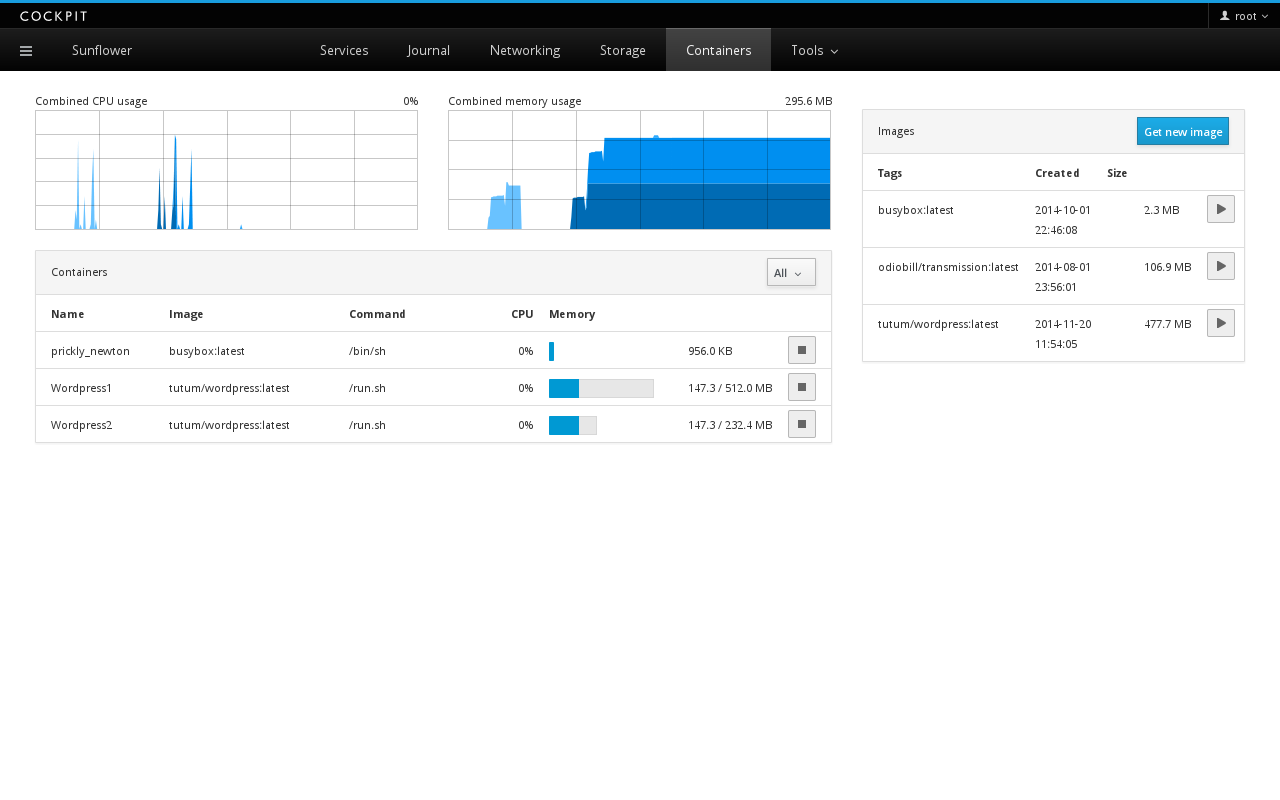
\includegraphics[keepaspectratio,width=\textwidth]{screenshot-docker.png}
\end{figure}
Cockpit is a server manager that makes it easy to administer your GNU/Linux servers via a web browser:
\begin{itemize}
  \item \textbf{Easy to use}: Cockpit is perfect for new sysadmins, allowing them to easily perform simple tasks such as storage administration, inspecting journals and starting and stopping services. 
  \item \textbf{No interference}: Jumping between the terminal and the web tool is no problem. A service started via Cockpit can be stopped via the terminal. Likewise, if an error occurs in the terminal, it can be seen in the Cockpit journal interface. 
  \item \textbf{Multi-server}: You can monitor and administer several servers at the same time.
\end{itemize}

\section{\textcolor{FedoraBlue}{Docker containers on armv7hl architecture}}
Users of the Fedora Server on armv7hl can now create and manage their own Docker containers!


\section{\textcolor{FedoraBlue}{Other improvements}}
\begin{itemize}
  \item Faster and better dependency management with \textbf{DNF}.
  \item \textbf{Ipsilon}: Ipsilon is a server and a toolkit to configure Apache-based Service Providers. The server is a pluggable self-contained mod\_wsgi application that provides federated SSO to web applications. User authentication is always performed against a separate Identity Management system (for example a FreeIPA server), and communication with application is done using a federation protocol like SAML, OpenID, etc.. 
  \item \ldots and much more
\end{itemize}

\section{\textcolor{FedoraBlue}{Exciting roadmap}}
The community continues to work towards making Fedora a better \href{http://www.gnu.org/philosophy/free-sw.en.html}{free} operating system for our users.

Information on the complete roadmap can be found here:\\ \href{http://fedoraproject.org/wiki/Releases/22/ChangeSet}{http://fedoraproject.org/wiki/Releases/22/ChangeSet}

%\vspace{1.5cm}
%\begin{figure}[h]
%  \centering
%  
\includegraphics[keepaspectratio]{Fedora-server-v5a-infinity.png}
%\end{figure}
\newpage

\begin{center}
  {\color{FedoraBlue}
  \LARGE{Fedora Project\vspace{1cm}}
  \Large{\href{http://fedoraproject.org}{http://fedoraproject.org}}
}
\end{center}

\section{\textcolor{FedoraBlue}{Getting Support}}
\subsection{Fedora project wiki and mailing lists}
\href{https://fedoraproject.org/wiki/Communicate}{https://fedoraproject.org/wiki/Communicate}

\subsection{Official Documentation}
\href{http://docs.fedoraproject.org}{http://docs.fedoraproject.org}

\subsection{IRC Channel}
\href{http://webchat.freenode.net/?channels=#fedora}{\#fedora @ irc.freenode.net}

\subsection{Community forums}
\href{http://ask.fedoraproject.org}{http://ask.fedoraproject.org}
\href{http://fedoraforum.org}{http://fedoraforum.org}


\section{\textcolor{FedoraBlue}{Looking to join the Fedora community?}}
Are you interested in contributing to Fedora? There are many ways you can become active in the project.  Whether you are a People Person, Designer, OS Developer, Packager or Administrator - we have a place for you. Just head to the following page and get started today!

\begin{center}\href{http://join.fedoraproject.org}{http://join.fedoraproject.org}\end{center}


\end{document}
